\section{Servidor}

Las partidas las maneja el objeto \texttt{Game}. Al crear el juego, debe recibir los jugadores (sockets) y el
\texttt{Stage} que debe crear. Este objeto consta de varios threads:

\begin{itemize}
    \item El gameloop.
    \item Un thread que lee de la entrada de cada cliente.
    \item Un thread que env\'ia los datos para cada cliente.
\end{itemize}


\subsection{Gameloop}

El game loop obtiene y ejecuta las acciones del jugador al cual le corresponde el turno, actualiza el motor de f\'isica,
serializa el nuevo estado del juego en un snapshot y duerme el tiempo necesario. El servidor es totalmente autoritario,
es decir, no acepta \'ordenes por parte del cliente, sino que recibe acciones y es \'el el que decide si son
aceptadas o no. El gameloop se actualiza en un framerate determinado (60 veces por segundo), con lo cual es importante
que pueda trabajar sin bloquearse en ninguna operacion, ya que afectar\'ia a todos los jugadores y arruinar\'ia la
experiencia de juego.


\subsection{Input workers}

Para evitar bloquear el gameloop, toda comunicaci\'on con los clientes se realiza mediante threads independientes. La acciones de los jugadores
son insertadas por los threads de entrada (\texttt{inputWorkers}) en una cola. Las colas utilizadas son
una objetos de tipo \texttt{Stream}, el cu\'al funciona como una cola protegida por un mutex que permite
hacer \texttt{pop} tanto en forma bloqueante o no bloqueante. El \texttt{Game} luego obtiene
en forma no bloqueante una acci\'on del jugador (cada uno tiene una cola asignada) y la procesa. Leer de forma
no bloqueante significa que, de no haber ninguna acci\'on del cliente encolada, se retorna \texttt{false} y
el gameloop continua con la ejecuci\'on. En caso que un cliente se desconecte, este thread realiza un \textt{push}
de un evento \textt{disconnect} en la cola, el cu\'al es leido por el gameloop cuando llega su turno, y maneja
el evento de la forma que corresponda.


\subsection{Output workers}

Al terminar una iteraci\'on, el estado del juego se almacena en un snapshot el cual es leido por threads
asignados a cada cliente (los \texttt{outputWorkers}), los cuales lo env\'ian serializado por el
socket correspondiente. Como cada snapshot tiene toda la informaci\'on sobre el estado juego
en un determinado momento, los \texttt{outputWorkers} solo necesitan enviar el mas reciente, por lo que no
es necesario utilizar una cola, sino que se usa un \texttt{DoubleBuffer}. Este objeto reserva memoria
para 2 copias de un objeto de un tipo determinado. En una de ellas (background copy) es en la que se escribe, y
la otra (current copy) puede ser leida al mismo tiempo. El escritor puede realizar un \texttt{swap} de las copias,
con lo que background se convierte en current. Para evitar problemas de concurrencia el \texttt{DoubleBuffer}
contiene un mutex que bloquea las operaciones \texttt{swap} mientras otro thread est\'e copiando al current.
Un thread puede bloquearse esperando un \texttt{swap} en un \texttt{DoubleBuffer}, lo cual permite que los
\texttt{outputWorkers} s\'olo envien datos cuando hay un nuevo snapshot disponible.


\section{Cliente}

El cliente tiene 3 threads:

\begin{itemize}
    \item El principal (renderer).
    \item El input worker.
    \item El output worker.
\end{itemize}


\subsection{Renderer}

Este thread es el encargado de dibujar el juego en la pantalla. Si bien maneja algunas animaciones client side,
mayormente dibuja el \'ultimo snapshot recibido del modelo. Es importante que este thread no se bloquee en ninguna
operaci\'on ya que dar\'ia la sensaci\'on de que el juego no responde. Es por esto que de no haber recibido un
snapshot nuevo, de todas formas continua ejecut\'andose y dubujando el \'ultimo recibido (adem\'as de continuar
actualizando las animaciones est\'eticas).

Otra tarea es la de obtener los eventos de SDL para procesarlos y actualizar animaciones. Esto no se realiza
en un thread independiente porque no es necesario ya que un ser humano no tiene la velocidad de generar demasiados
eventos en una iteracion de forma que se pudiera demorar proces\'andolos. Esto resulta una ventaja porque de esta
forma no es necesaria la utilizaci\'on de threads (y mutex) en el render loop, minimizando los posibles errores
y la complejidad del mismo.


\subsection{Input worker}

Este thread obtiene de la conexi\'on con el servidor los nuevos snapshots. De forma similar a como trabaja el servidor,
este thread almacena los snapshots en un \texttt{DoubleBuffer}, con la diferencia de que el \texttt{Renderer} no
se bloquea esperando un \textt{swap}, sino que siempre obtiene una copia (aunque sea una ya leida previamente).


\subsection{Output worker}

El cliente debe enviar las acciones del cliente al servidor mediante el socket. Para evitar bloquearse en un \textt{send},
esta tarea es realizada por un thread. La comunicaci\'on entre este thread y el renderer se realiza mediante un
\textt{Stream}. El renderer hace \textt{push} y este thread hace un \textt{pop} bloqueante para evitar un busy wait.
Cada acci\'on es luego serializada y enviada al servidor.


El siguiente esquema muestra la comunicaci\'on entre un cliente y el servidor. Cada flecha vertical representa un thread
en el proceso en el cual se origina, mientras que las flechas horizontales indican comunicaci\'on de alguna forma:

\begin{figure}
\begin{center}
\subfloat[]{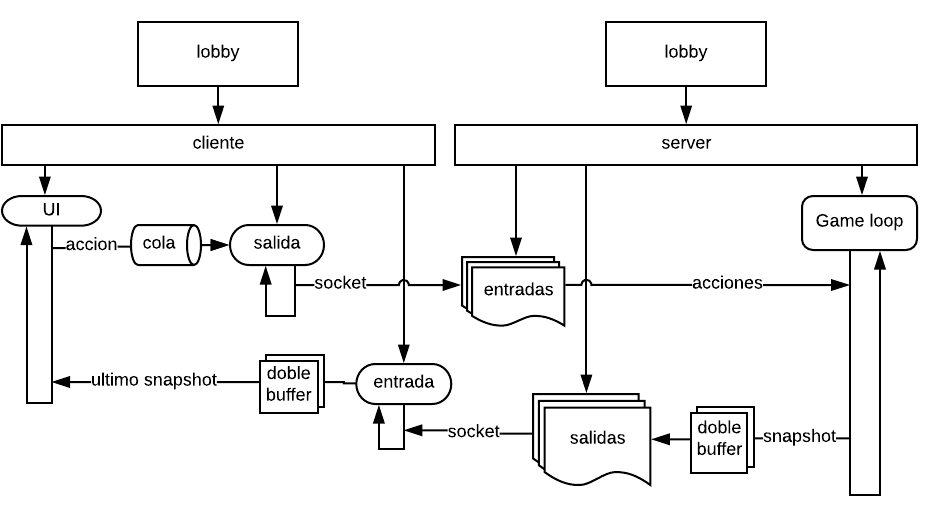
\includegraphics[width=\textwidth,height=\textheight,keepaspectratio]{img/gameCommunication.png}}
\end{center}
\end{figure}


\section{Conclusiones sobre la comunicaci\'on}

El modelo implementado result\'o exitoso, ya que no provoc\'o problemas durante el desarrollo de la l\'ogica del juego
y permite una experiencia de juego satisfactoria. Encapsula la concurrencia en peque\~os objetos que manejan la
comunicaci\'on sin mayores dificultades.
